\documentclass[preprint,12pt]{elsarticle}
\usepackage[T1]{fontenc}
\usepackage[utf8]{inputenc}
\usepackage[brazil]{babel}
\usepackage{amsmath,amssymb,booktabs,graphicx}
\usepackage{xurl}
\usepackage{placeins}
\setlength{\emergencystretch}{2em}
\renewcommand{\floatpagefraction}{0.8}
\renewcommand{\topfraction}{0.9}
\renewcommand{\textfraction}{0.1}
\usepackage[hidelinks]{hyperref}
\journal{Supply Chain Analytics -- versão de trabalho em português}
\begin{document}
\begin{frontmatter}
\title{Seleção de políticas de reposição por perfil de demanda: avaliação temporal em uma rede varejista}
\author[ufal]{Matheus Inácio Batista Santos}
\affiliation[ufal]{organization={Instituto de Computação, Universidade Federal de Alagoas},country={Brasil}}
\begin{abstract}
A heterogeneidade da demanda motiva selecionar políticas de reposição por perfil, mas essa complexidade só se justifica se melhorar a decisão em períodos posteriores. Este estudo compara seleção por perfil e política global em 145 séries loja-produto de uma rede varejista brasileira, distribuídas em 115 lojas e nove produtos. Avaliamos seis políticas principais e DQN como controle adicional, em duas origens temporais, com blocos separados de treino, validação e teste. Os métodos estocásticos usam três sementes, totalizando 4.350 ajustes. Em cada origem, a escolha minimiza custo entre candidatas que atingem atendimento médio mínimo de 0,70 na validação das demais lojas; o desempenho é medido no teste da loja reservada. A seleção por perfil aumenta o custo médio em 1,93\% e o atendimento em 3,89 pontos percentuais. Os casos abaixo da meta diminuem de 119 para 100 entre 283 casos série--origem com demanda positiva; sete casos têm atendimento indefinido. O intervalo condicional de 95\% para o aumento de custo é de $[-0{,}32;4{,}16]\%$. A diferença concentra-se na primeira origem; na segunda, ambos os seletores escolhem a mesma política. Os resultados mostram serviço adicional com custo maior, sem economia geral da seleção contextual. A coorte retrospectiva e duas janelas curtas parcialmente sobrepostas limitam a generalização.
\end{abstract}
\begin{keyword}
Gestão de estoques \sep Demanda intermitente \sep Seleção de políticas \sep Nível de serviço \sep Varejo \sep M5
\end{keyword}
\end{frontmatter}

\section{Introdução}
Uma rede varejista precisa decidir quando e quanto repor para muitas combinações de loja e produto. Uma regra que funciona para vendas frequentes pode produzir excesso de estoque em séries esparsas; outra, econômica em média, pode não cobrir picos relevantes. O problema não se resume a prever demanda: envolve escolher uma regra de decisão e ajustar seus parâmetros sob custos e exigências de atendimento \cite{Axsater2006InventoryControl}.

Comparações de algoritmos ampliam o conjunto de alternativas disponíveis. Políticas analíticas, heurísticas, busca por parâmetros e aprendizado por reforço oferecem diferentes compromissos entre custo, serviço e esforço computacional. Entretanto, a existência de um portfólio não resolve a escolha operacional. O gestor precisa saber se vale aplicar uma política uniforme ou distinguir grupos de séries, e se a distinção oferece ganho suficiente para justificar maior complexidade.

Essa pergunta pode ser formulada como seleção de algoritmos: características de uma instância ajudam a escolher um método de um conjunto candidato \cite{rice1976,Kotthoff2014AlgorithmSelection}. Em inventário, a instância é uma série loja-produto e o resultado depende da política, do ambiente e do serviço exigido. A proposta Adaptive Inventory Policy Engine (AIPE) organiza essa avaliação em caracterização, comparação e seleção. Seu componente supervisionado, Policy Selection Engine (PSE), é uma extensão ainda não validada neste artigo; a análise presente utiliza regras explícitas de escolha por perfil.

Trabalhos publicados em \textit{Supply Chain Analytics} relacionam previsão e desempenho operacional \cite{sca_f81ad2b3e023}, comparam algoritmos de controle \cite{sca_27e994c54848} e examinam a informação decisória preservada por critérios de classificação \cite{sca_c5c06dcbc9e5}. Esses enfoques motivam avaliar o que a seleção por perfil acrescenta ao portfólio: distinguir padrões de demanda só justifica uma regra mais complexa se a distinção melhorar a decisão em relação a uma referência global competitiva.

O artigo concentra-se em uma pergunta: selecionar políticas por perfil de demanda melhora o compromisso entre custo e atendimento frente à seleção de uma política global? As duas estratégias usam a mesma informação passada e o mesmo portfólio. A avaliação combina dados de uma rede brasileira e um conjunto público de varejo, mantendo as bases separadas. Neste estágio, a matriz da Bahia está completa e a execução M5 está em andamento; apenas resultados completos sustentam conclusões quantitativas.

Três análises sustentam essa pergunta: o compromisso custo--serviço das candidatas; a diferença entre seleção global e por perfil no teste; e a estabilidade das escolhas e do atendimento entre origens temporais. A comparação de controladores serve para interpretar a seleção, sem constituir uma segunda proposta de algoritmo. O estudo não pretende abranger todos os componentes do AIPE nem validar seu seletor supervisionado.

\section{Trabalhos relacionados e posicionamento}
A classificação da demanda organiza diferenças de frequência e tamanho das ocorrências. A taxonomia ADI--CV$^2$ é uma referência para distinguir demanda suave, errática, intermitente e \textit{lumpy} \cite{syntetos2005}. Uma classe estatística, porém, não identifica sozinha a melhor política: custo de falta, prazo, estado inicial e requisito de atendimento também influenciam a decisão.

Tadayonrad e Ndiaye \cite{sca_f81ad2b3e023} aproximam a avaliação de previsão dos custos de inventário e do serviço. Pietukhov et al.\ \cite{sca_92a549559870} estudam previsão de indicadores de desempenho em um contexto empírico. A conexão com este trabalho é avaliar consequências operacionais, sem transformar precisão preditiva em substituto de custo e atendimento. Na avaliação principal, previsão especializada não é uma intervenção experimental; a escolha é julgada pelas decisões e pelo serviço obtido.

Zabraoui et al.\ \cite{sca_27e994c54848} comparam famílias de algoritmos de inventário e apresentam combinações de algoritmos genéticos (GA) e aprendizado por reforço com dados M5. A arquitetura GA--DQN, que combina GA e uma rede Q profunda (DQN, do inglês deep Q-network), e a ideia de portfólio já estão, portanto, na literatura da revista. Nosso foco não é propor a mesma combinação como novidade, mas avaliar a camada de escolha entre alternativas. As heurísticas inspiradas naquele estudo envolvem decisões de implementação próprias, e custos, filtros e granularidade não constituem uma reprodução exata de seus experimentos.

A análise de critérios de Theunissen et al.\ \cite{sca_c5c06dcbc9e5} destaca a diferença entre importância estatística e utilidade decisória. Não implementamos seu método topológico. Testamos uma consequência próxima: mesmo um perfil interpretável pode ser pouco útil se recomendar praticamente a mesma política global ou se suas mudanças elevarem custo sem benefício de serviço relevante.

Revisões de aprendizado por reforço em inventário discutem a importância do ambiente, da recompensa e da avaliação \cite{Boute2022DRLInventoryRoadmap}. Uma baixa taxa de atendimento ou frequência de pedidos extrema não caracteriza, isoladamente, uma família algorítmica. Os resultados abaixo descrevem implementações e matrizes específicas. A interpretação exige identificar o controlador, seu orçamento e as condições comuns de avaliação.

O M5 documenta uma competição de previsão sobre vendas reais de varejo \cite{Makridakis2022M5Accuracy}. Neste artigo, seus dados são agregados e usados em simulação de reposição. Os resultados não são classificações da competição nem uma comparação com seus vencedores. O conjunto público permite investigar a mesma pergunta de seleção em outro contexto, com protocolo explicitado por base e sem comparar custos absolutos entre bases.

\section{Dados e protocolo temporal da Bahia}
\label{sec:ba2026_methods}

A avaliação utiliza 145 séries loja--produto da Bahia, em 115 lojas e nove produtos, com 38 ciclos comerciais disponíveis, identificados de 202301 a 202504. Os ciclos são unidades comerciais da fonte; não representam observações diárias. O objetivo é comparar uma política global com a escolha por perfil em períodos posteriores aos usados no ajuste e na seleção. A coorte foi definida retrospectivamente; os ajustes e a seleção, porém, utilizam apenas a informação disponível antes do teste. Essa distinção limita a generalização para séries ainda não observadas.

\subsection{Protocolo e cobertura}

Os registros complementares de vendas são somados por chave, sem descartar transações apenas por compartilharem loja, produto e ciclo. A coorte tem identificadores fixos; em cada origem, exige ao menos três ciclos positivos no treino. As 145 séries são elegíveis nos dois prefixos, de 17 e 23 ciclos. Cada prefixo é seguido por sete ciclos de validação e sete de teste. Na numeração iniciada em um, os testes abrangem os ciclos 25--31 e 31--37: compartilham um ciclo e representam medidas repetidas das mesmas séries.

Perfis, escalas dos estados e parâmetros são calculados no treino. O prazo efetivo de entrega é de dois ciclos, e EOQCycle utiliza demanda e manutenção na mesma unidade temporal. Custos de manutenção, falta, emissão e quantidade permanecem, respectivamente, em 1 por unidade e ciclo, 5 por unidade não atendida, 50 por pedido e 0,5 por unidade pedida. São unidades do cenário, sem equivalência monetária calibrada. O custo soma manutenção, falta e pedidos no bloco de teste, sem crédito pelo estoque final. Estados iniciais comuns são obtidos por uma política EOQ de referência: um aquecimento no passado precede a validação, e sua trajetória na validação determina o estado inicial do teste. O teste não continua o estoque particular de cada candidata.

O portfólio contém EOQCycle, sSCycle, CappedBaseStock, GA, PPO, GA--DQN e DQN. O último é o controle do híbrido e também está disponível à regra de seleção. As três primeiras políticas têm um ajuste por série e origem. GA, PPO, GA--DQN e DQN usam sementes 11, 29 e 47, totalizando 4.350 ajustes e 8.700 registros de validação ou teste. A matriz está completa, sem casos excluídos por falta de política ou semente. O GA usa população de 100 indivíduos e 50 gerações. DQN e PPO têm orçamento mínimo de 20 mil transições, arredondado para episódios completos: 20.009 e 20.010 nas duas origens. GA--DQN acrescenta busca genética e mil transições de demonstração; seu esforço total é maior que o do DQN isolado. A variante avaliada mantém o mesmo gatilho e piso de pedido nas demonstrações, no treinamento e na inferência.

As sementes são primeiro promediadas dentro de cada série, origem e política. Para cada loja excluída, as políticas global e por perfil são escolhidas na validação das demais lojas e avaliadas no teste da loja reservada. O limiar principal é 0,70. Escolher uma alternativa viável na validação não garante repetir seu atendimento no futuro. Se nenhuma candidata cumpre a meta, a escolha de maior serviço é registrada como alternativa de contingência, sem classificá-la como viável.


\subsection{Sistema de estoque, métricas e candidatas}

Cada série é simulada separadamente em um sistema de vendas perdidas: demanda não atendida no ciclo não se transforma em pedido pendente. Não há estoque compartilhado entre lojas, capacidade conjunta ou transbordo. O simulador admite quantidades não negativas sem impor arredondamento a unidades inteiras ou lotes mínimos de compra. A política decide com o estado anterior ao recebimento do ciclo; a entrega respeita o prazo exato de dois ciclos. O recebimento precede a demanda, e manutenção incide sobre o saldo após o atendimento.

Para o teste de sete ciclos, o custo é
\begin{equation}
C=\sum_t\left[hI_t+p(d_t-v_t)+K\mathbf{1}(q_t>0)+cq_t\right],
\end{equation}
em que $I_t$ é o estoque após a demanda, $d_t$ a demanda observada, $v_t$ a quantidade atendida e $q_t$ o pedido emitido. Os coeficientes são $h=1$, $p=5$, $K=50$ e $c=0{,}5$. Pedidos em trânsito não atendem demanda antes da chegada. O custo reportado não contém as penalidades auxiliares usadas no treino.

\begin{table}[htbp]\centering\small
\caption{Candidatas e decisões implementadas. Parâmetros e escalas usam somente o treino da própria série.}
\label{tab:implemented_policies}
\begin{tabular}{@{}p{3.2cm}p{7.6cm}@{}}\toprule
Candidata & Regra e ajuste\\\midrule
EOQCycle & Lote fixo ao atingir o ponto de pedido; lote EOQ por ciclo e proteção com $z=1{,}28$.\\
sSCycle & Mesmo ponto de pedido, com reposição até o ponto acrescido do lote EOQ; parâmetros analíticos, sem otimização exata de $(s,S)$.\\
CappedBaseStock & Reposição até um alvo com teto de quantidade; busca determinística em grade de $20\times12$ pares.\\
GA & Busca evolutiva de ponto de pedido, lote e proteção adicional.\\
DQN & Rede Q profunda, variante Double DQN com arquitetura dueling, para escolher entre 20 quantidades discretas.\\
PPO & Otimização proximal de políticas, com 20 ações discretas e estimação generalizada de vantagem.\\
GA--DQN & DQN com demonstrações, gatilho e piso de pedido derivados do GA.\\
\bottomrule\end{tabular}
\end{table}
\FloatBarrier

A Tabela~\ref{tab:implemented_policies} identifica as implementações que compõem o portfólio. Nas referências analíticas, $Q=\max(1,\sqrt{2\mu K/h})$ e $r=2\mu+1{,}28\sigma\sqrt{2}$, em que $\mu$ e $\sigma$ são média e desvio-padrão populacional do treino. EOQCycle pede $Q$ quando a posição de estoque não excede $r$; sSCycle repõe até $r+Q$. CappedBaseStock usa $q_t=\min(u,\max(0,S-\mathrm{IP}_t))$, com alvo $S$, teto $u$ e posição de estoque $\mathrm{IP}_t$.

DQN e PPO usam duas camadas de 64 unidades. O estado tem seis componentes: estoque, previsão ingênua, pedidos em trânsito, média e dispersão dos últimos seis ciclos e posição no horizonte. As escalas vêm do treino e o estado usa apenas observações passadas. No híbrido, a quantidade é zero acima do gatilho genético; abaixo dele, é o máximo entre a ação da rede e metade do lote genético. Essa transformação é mantida em demonstração, treino e aplicação.

Os objetivos de calibração não são idênticos. GA minimiza custo acrescido de penalidade pelo déficit de atendimento frente a 0,70. Os agentes usam recompensa de custo negativo e penalidade terminal pelo mesmo déficit. A escala da penalidade é $30\max(5\sum_t d_t,1)$. CappedBaseStock acrescenta termos de frequência de ruptura e amplificação da variância dos pedidos, com peso unitário, que não são usados pelo GA. Essa diferença precisa acompanhar a leitura do ranking: a avaliação compara as candidatas configuradas, sem isolar a qualidade de suas famílias ou igualar todos os esforços de ajuste.

\begin{figure}[htbp]
\centering
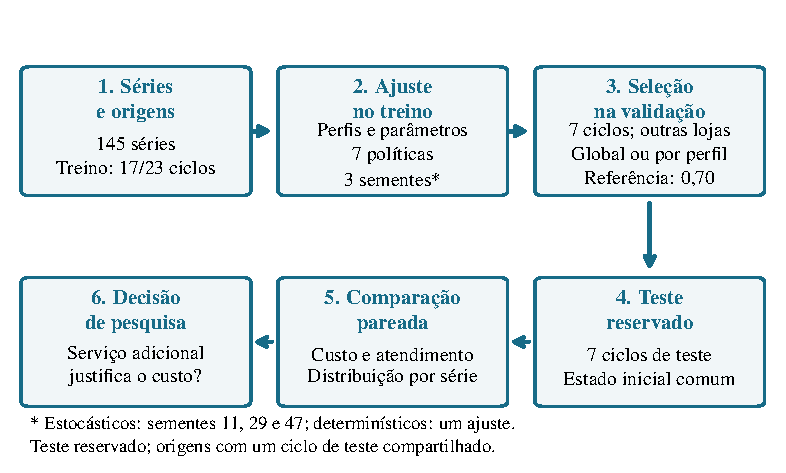
\includegraphics[width=\linewidth]{figures/fluxo_experimental.pdf}
\caption{Fluxo da avaliação e separação da informação. Cada candidata é ajustada no treino da própria série. A estratégia de seleção usa a validação das demais lojas e é avaliada no teste da loja reservada. Os dois testes compartilham um ciclo; as origens são medidas repetidas.}
\label{fig:experimental_flow}
\end{figure}

O fluxo da Figura~\ref{fig:experimental_flow} mantém separadas duas decisões: ajustar o controlador e escolher qual controlador recomendar. Para cada caso, o atendimento é $F=\sum_t v_t/\sum_t d_t$, em que $v_t$ é a demanda atendida e $d_t$ a demanda observada. Quando o denominador é zero, $F$ permanece indefinido. A média por caso atribui peso igual às séries com demanda; o atendimento ponderado usa a razão entre todas as unidades atendidas e demandadas. Ambos acompanham o custo total, para evitar que baixo atendimento seja interpretado como eficiência econômica.


\section{Seleção e protocolo de comparação}
\subsection{Referência global e escolha por perfil}
Para um conjunto $A$ de séries usadas na escolha, definimos custo e atendimento médios por política:
\begin{equation}
 \bar C_{\pi,A}=|A|^{-1}\sum_{i\in A}C_{i\pi},\qquad
 \bar F_{\pi,A}=|A|^{-1}\sum_{i\in A}F_{i\pi}.
\end{equation}
Cada série recebe o mesmo peso. A média de fill rates não é o atendimento ponderado pelo volume total da rede. Seja $\Pi$ o portfólio de políticas. A política global é
\begin{equation}
 \widehat\pi_A=\arg\min_{\pi\in\Pi:\bar F_{\pi,A}\geq\alpha}\bar C_{\pi,A}.
\end{equation}
A seleção por perfil aplica a mesma regra separadamente a $A_g$, o subconjunto associado ao perfil $g$. Se nenhuma política atende à restrição, escolhe-se maior atendimento médio, com custo como desempate, e registra-se fallback. Esse caso é explicitado: não é uma escolha viável que cumpriu o limiar. Entre candidatas viáveis com mesmo custo, preferimos maior serviço; no fallback empatado em serviço, menor custo. Empates restantes usam ordem alfabética do identificador. Um perfil ausente nas lojas de escolha utiliza a regra global.

A restrição é média e específica do conjunto usado para escolher. Não exige $F_{i\pi}\geq\alpha$ em toda série. Também não garante a média da loja excluída. Além disso, exigir viabilidade em cada perfil é diferente de exigi-la apenas no agregado. Uma política global viável pode ser inviável em um grupo; a escolha por perfil não precisa apresentar menor custo mesmo na avaliação retrospectiva.

O limiar principal é $\alpha=0{,}70$, herdado da investigação original. Ele não representa recomendação de meta comercial. Avaliamos também 0,80, 0,85, 0,90 e 0,95, sem escolher a conclusão pelo limiar mais favorável. A diferença relativa de custo é
\begin{equation}
 R=100\frac{\bar C_{\mathrm{global}}-\bar C_{\mathrm{perfil}}}{\bar C_{\mathrm{global}}}.
\end{equation}
$R>0$ indica redução; $R<0$, aumento. Diferenças de atendimento são dadas em pontos percentuais. Custo menor acompanhado por atendimento menor não é chamado de dominância.

\subsection{Perfis operacionais e informação disponível}
Os perfis são regras heurísticas ordenadas, não clusters aprendidos nem políticas previamente validadas. A prioridade é Sparse High Impact, High Volatility Seasonal, Unstable Trend, Low Volume Stable e Fast Moving. A primeira regra utiliza ADI elevado, CV$^2$ elevado e sequência longa de zeros; a segunda, autocorrelação sazonal ou concentração de ocorrências; a terceira, tendência ou entropia. Os perfis de baixo volume estável e venda frequente não aparecem nos prefixos avaliados da Bahia. Para tornar a regra reproduzível, usamos $a=n/\max(n_+,1)$, $c^2=[s/(\mu+10^{-9})]^2$ e $Z$, maior sequência de zeros. Aqui, $n$ é o número de ciclos do prefixo de treino, $n_+$ é a quantidade de ciclos com demanda positiva, $\mu$ é a média sobre todos os ciclos e $s$ é o desvio-padrão amostral, incluindo zeros. Essa variância difere da calculada apenas sobre os tamanhos positivos da demanda na taxonomia original. A Tabela~\ref{tab:profile_rules} apresenta os cortes, aplicados na ordem indicada; uma série sem correspondência recebe Sparse High Impact.

\begin{table}[htbp]\centering\small
\caption{Regras operacionais de perfil: primeiro corte satisfeito determina o grupo.}\label{tab:profile_rules}
\begin{tabular}{@{}p{3.7cm}p{7.2cm}@{}}\toprule
Perfil & Condição\\\midrule
Sparse High Impact & $a\geq1{,}32$, $c^2\geq0{,}49$ e $Z\geq5$\\
High Volatility Seasonal & Autocorrelação na defasagem 17 $\geq0{,}25$ ou burstiness $\geq0{,}30$\\
Unstable Trend & Módulo da tendência normalizada $\geq0{,}05$ ou entropia $\geq2$\\
Low Volume Stable & $\mu\leq2$ e $c^2<0{,}49$\\
Fast Moving & $a<1{,}32$\\\bottomrule\end{tabular}\end{table}

Burstiness é $(s_\Delta-\mu_\Delta)/(s_\Delta+\mu_\Delta+10^{-9})$, em que $\mu_\Delta$ e $s_\Delta$ são a média e o desvio-padrão dos intervalos $\Delta$ entre ocorrências positivas; recebe zero com menos de dois intervalos. Tendência é a inclinação estimada por mínimos quadrados ordinários (OLS) sobre o índice de ciclo, dividida por $\mu+10^{-9}$. Entropia é $-\sum_j p_j\log_2(p_j+10^{-12})$, em que $p_j$ é a frequência relativa na classe $j$ de um histograma com dez intervalos de mesma largura. Autocorrelação é a covariância na defasagem 17 dividida pela variância global; recebe zero se a série tem até 18 ciclos ou variância desprezível. Os rótulos descrevem regras locais, não sazonalidade ou impacto econômico empiricamente validados.

Na avaliação temporal, essas características são calculadas exclusivamente no prefixo de treino. Os nomes dos perfis identificam regras locais; não validam sazonalidade ou impacto econômico. A eventual associação de um nome de perfil a uma política no código não determina a escolha: custo e serviço na validação definem a recomendação.

\subsection{Avaliação e incerteza}
As regras global e por perfil usam a validação das demais lojas e são aplicadas ao teste da loja reservada. Cada política é ajustada apenas no treino da respectiva série; o seletor usa resultados de validação, sem consultar o teste para escolher. As sementes são promediadas dentro de cada caso série--origem antes das comparações. Custos incluem todos os casos; médias de atendimento excluem os denominadores nulos, contabilizados separadamente. Origens são medidas repetidas, com um ciclo de teste compartilhado.

A incerteza de custo é descrita por intervalos percentis de 95\%, obtidos em 5.000 reamostragens pareadas das 115 lojas. Cada loja sorteada leva todas as suas séries e origens. Controladores e seletores permanecem fixos nos sorteios; os intervalos são condicionais às escolhas e aos treinamentos realizados. A dependência entre lojas que compartilham produtos permanece uma limitação.

\section{Resultados: valor da seleção por perfil}
\label{sec:ba2026}

\subsection{Quais candidatas oferecem compromissos competitivos?}

A Tabela~\ref{tab:ba2026_portfolio} resume os 290 casos série--origem. Sete casos não têm demanda no teste: um na primeira origem e seis na segunda. Seus custos permanecem na média dos 290 casos; o atendimento médio utiliza os 283 casos com denominador positivo. O atendimento ponderado é a razão entre a soma das unidades atendidas e a soma da demanda nos blocos avaliados, após a média das sementes. As origens repetidas não ampliam a amostra para 290 séries independentes.

\begin{table}[htbp]
\centering\small
\caption{Bahia, protocolo temporal: médias no teste de sete ciclos. Custo em unidades do cenário, calculado nos 290 casos. Atendimento médio e contagem abaixo da meta consideram os 283 casos com demanda positiva; sete casos têm atendimento indefinido.}
\label{tab:ba2026_portfolio}
\begin{tabular}{@{}lrrrr@{}}\toprule
Política & Custo & Atendimento & Ponderado & Abaixo de 0,70\\\midrule
EOQCycle &166,77&0,7787&0,6265&101\\
sSCycle &164,23&0,8037&0,6802&90\\
CappedBaseStock &218,11&0,6631&0,4948&148\\
GA &143,85&0,6953&0,5457&140\\
PPO &134,23&0,5514&0,4189&171\\
GA--DQN &145,75&0,6802&0,5248&144\\
DQN (controle) &164,88&0,5718&0,4033&164\\
\bottomrule\end{tabular}
\end{table}

PPO tem o menor custo descritivo, acompanhado do menor atendimento médio. Apenas EOQCycle e sSCycle superam 0,70 no conjunto dos testes; nenhuma política alcança essa meta no atendimento ponderado. Entre essas duas referências, sSCycle apresenta menor custo e maior atendimento médio. Essa comparação é um diagnóstico do teste, não uma escolha retrospectiva a ser atribuída ao seletor.

GA--DQN custa 11,60\% menos que DQN e aumenta o atendimento médio de 0,5718 para 0,6802. Frente ao GA isolado, porém, custa 1,32\% mais e atende menos, com média de 0,6953 para o GA. O refinamento híbrido não oferece vantagem agregada nessas duas dimensões sobre seu componente evolutivo. A diferença varia entre origens: na segunda, seu custo é ligeiramente menor que o do GA, também com menor atendimento. A comparação descreve o comportamento das implementações avaliadas, sem isolar causalmente o benefício das demonstrações ou do gatilho.

\begin{figure}[htbp]
\centering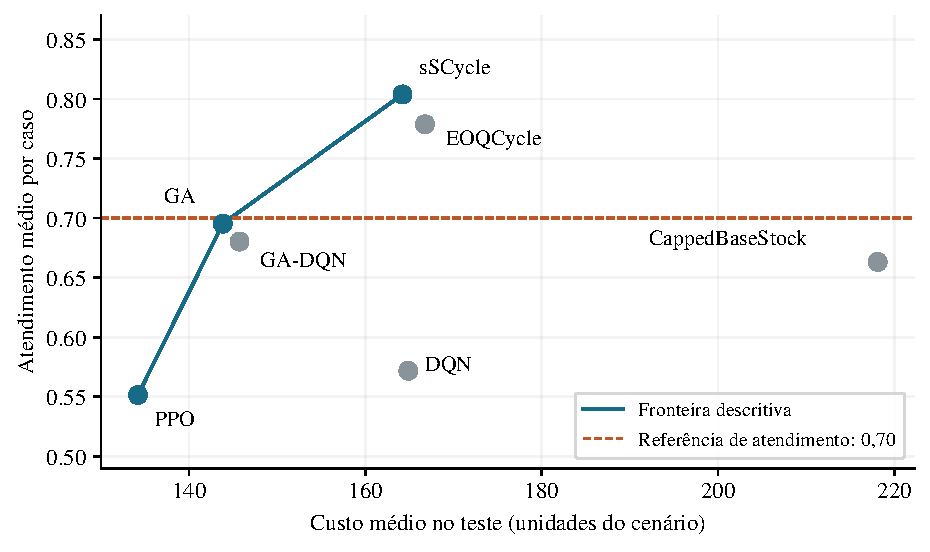
\includegraphics[width=\linewidth]{figures/custo_servico.pdf}
\caption{Compromisso custo--serviço das sete candidatas na Bahia. Médias de teste em 290 casos série--origem para custo e 283 com demanda positiva para atendimento. A fronteira é descritiva: não utiliza o teste para escolher a recomendação nem representa dominância estatística ou por série.}
\label{fig:cost_service}
\end{figure}

A Figura~\ref{fig:cost_service} distingue economia aparente por baixo atendimento de um compromisso competitivo. A restrição usada pelo seletor continua sendo avaliada na validação, sem recorrer a essa fronteira de teste.

\subsection{O perfil melhora a decisão frente à seleção global?}

\begin{table}[htbp]
\centering\small
\caption{Escolha na validação das demais lojas e avaliação no teste da loja reservada, com meta 0,70. Há 145 casos por linha; atendimento definido em 144 casos na origem 17 e 139 na origem 23.}
\label{tab:ba2026_selection}
\begin{tabular}{@{}llrrr@{}}\toprule
Treino & Estratégia & Custo & Atendimento & Abaixo de 0,70\\\midrule
17 ciclos & Global &180,58&0,5711&101\\
17 ciclos & Perfil &186,79&0,6475&82\\
23 ciclos & Global &142,03&0,9073&18\\
23 ciclos & Perfil &142,03&0,9073&18\\
\bottomrule\end{tabular}
\end{table}

Na primeira origem, a regra global escolhe GA para todas as séries. Por perfil, as escolhas são GA em 65 casos, sSCycle em 75 e EOQCycle em cinco. O maior atendimento custa mais, e ambas as estratégias ficam abaixo da meta no teste. Na segunda origem, os dois seletores escolhem sSCycle em todos os casos. A Tabela~\ref{tab:ba2026_selection} evidencia, portanto, tanto mudança temporal da escolha global quanto ausência de diferenciação contextual na segunda janela.

No conjunto das origens, o custo médio passa de 161,31 na estratégia global para 164,41 por perfil: aumento de 1,93\%. O atendimento médio cresce de 0,7362 para 0,7751, diferença de 3,89 pontos percentuais; o ponderado passa de 0,5750 para 0,6395. Os casos abaixo da meta diminuem de 119 para 100, entre os 283 com atendimento definido. A estimativa pontual combina custo maior e melhor serviço, com a diferença concentrada na primeira origem. Essa melhora não assegura atendimento mínimo individual nem equivale a cumprir uma meta ponderada de 0,70.

Uma reamostragem exploratória pareada de 115 lojas, com 5.000 sorteios e todas as origens e produtos de cada loja preservados, produz intervalo condicional de 95\% de $[-0{,}32;4{,}16]\%$ para o aumento de custo por perfil. Os controladores e seletores permanecem fixos nos sorteios. Para a diferença de atendimento, o mesmo procedimento produz $[2{,}78;5{,}07]$ pontos percentuais. O intervalo de custo inclui zero; o de atendimento permanece positivo. Ambos são condicionais e não representam incerteza de novos treinamentos ou de novas trajetórias de demanda; dependência entre lojas que compartilham produtos também permanece possível.

\subsection{Sensibilidade ao limiar de escolha}

A Tabela~\ref{tab:threshold_sensitivity} apresenta todos os limiares avaliados. Em 0,80, a estratégia por perfil tem atendimento médio ligeiramente menor e custo maior que a global. Em 0,85, ambas selecionam sSCycle nos 290 casos, embora a frequência de contingência seja diferente: uma escolha pode cumprir o critério de seu grupo e não cumprir o critério agregado, ou o contrário. Em 0,90 e 0,95, ambas usam contingências em todos os casos. Portanto, a diferenciação contextual não preserva a vantagem de atendimento em todas as metas.

\begin{table}[htbp]\centering\small
\caption{Sensibilidade da seleção, sem retreinamento. Custo em 290 casos; atendimento médio em 283. Contingências indicam ausência de candidata viável na validação; não informam cumprimento de serviço no teste. G: global; P: por perfil.}
\label{tab:threshold_sensitivity}
\begin{tabular}{@{}rrrrrr@{}}\toprule
Meta & Custo G & Custo P & Atend. G & Atend. P & Conting. G/P\\\midrule
0,70 &161,31&164,41&0,7362&0,7751&0/0\\
0,80 &164,33&164,53&0,8037&0,8025&145/223\\
0,85 &164,23&164,23&0,8037&0,8037&290/225\\
0,90 &164,23&164,23&0,8037&0,8037&290/290\\
0,95 &164,23&164,23&0,8037&0,8037&290/290\\
\bottomrule\end{tabular}
\end{table}

As candidatas continuam calibradas com referência de 0,70. A inexistência de uma opção viável em uma meta maior não demonstra impossibilidade de atendê-la com outro ajuste ou portfólio. A sensibilidade examina a regra de seleção sobre a matriz disponível.

\begin{figure}[htbp]
\centering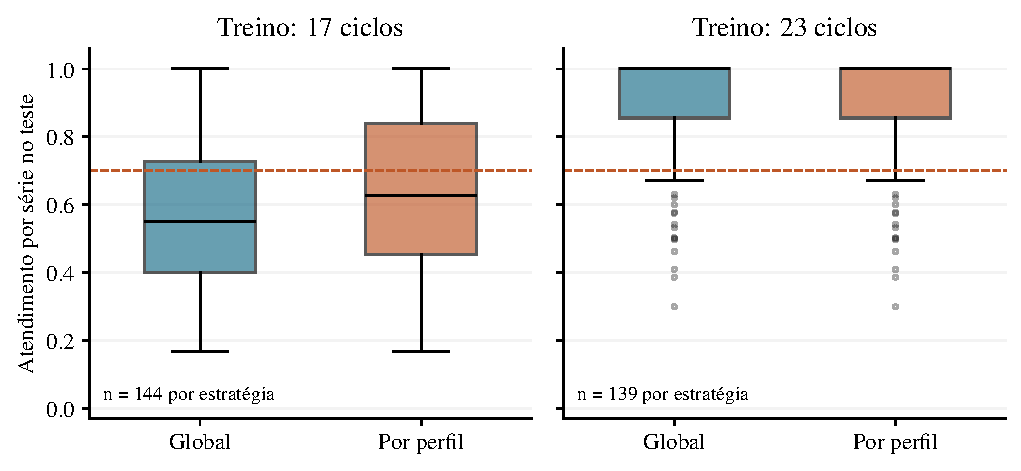
\includegraphics[width=\linewidth]{figures/distribuicao_atendimento.pdf}
\caption{Distribuição do atendimento das estratégias no teste, por origem. Cada caixa resume séries com demanda positiva; a linha tracejada indica 0,70. Há 144 casos por estratégia na primeira origem e 139 na segunda. As mesmas séries participam das duas estratégias; observações e origens não são independentes.}
\label{fig:service_distribution}
\end{figure}

A Figura~\ref{fig:service_distribution} mostra por que a comparação não se esgota na média: a primeira janela concentra violações de serviço, enquanto a segunda tem distribuição e escolha coincidentes entre estratégias.

\subsection{As escolhas e o atendimento são estáveis entre períodos?}

Os perfis são recalculados no prefixo disponível em cada origem. Com 17 ciclos, há 65 séries Sparse High Impact e 80 Unstable Trend; com 23, são 60, 69 e 16 High Volatility Seasonal. Essa mudança reflete a janela e as regras de caracterização, inclusive a indisponibilidade da autocorrelação na primeira origem. Não demonstra mudança de regime econômico em todas essas séries.


\begin{figure}[htbp]
\centering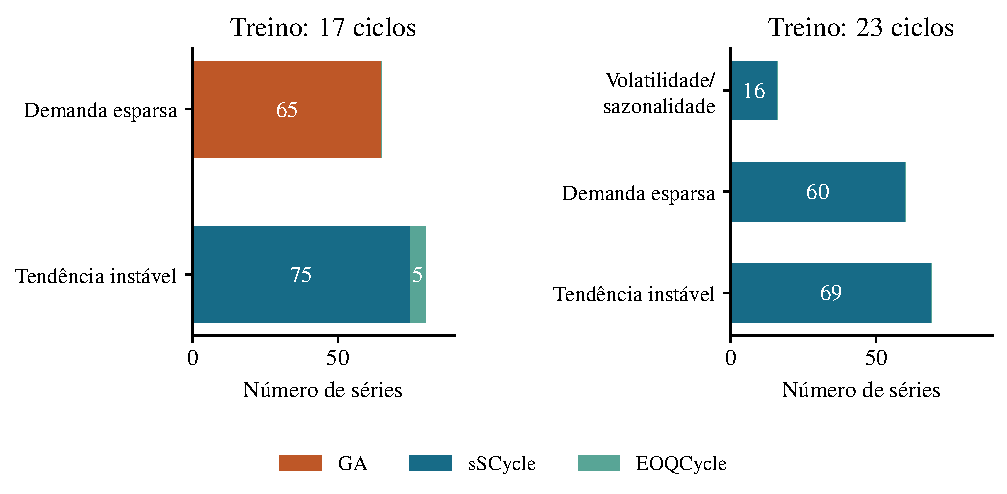
\includegraphics[width=\linewidth]{figures/escolhas_perfil.pdf}
\caption{Políticas escolhidas por perfil na validação das demais lojas, com meta 0,70. Cada painel contém 145 escolhas; os números indicam séries. A primeira origem diferencia grupos, enquanto a segunda recomenda sSCycle em todos eles. Nomes abreviados dos perfis correspondem às regras operacionais descritas no método.}
\label{fig:profile_choices}
\end{figure}

A Figura~\ref{fig:profile_choices} localiza a diferenciação que produz o serviço adicional: na primeira origem, a regra por perfil substitui GA por sSCycle ou EOQCycle em parte das séries. Na segunda, identificar perfis não muda a política recomendada. Assim, a existência de grupos distintos não implica valor incremental da seleção em todo período.
\FloatBarrier


\section{Discussão e implicações operacionais}
A avaliação temporal responde à pergunta central com um compromisso: os perfis aumentam o atendimento, mas também o custo. A melhora concentra-se na primeira origem, enquanto a segunda reproduz integralmente a escolha global. Não há evidência de economia geral que justifique, por si só, a complexidade adicional da seleção contextual.

Essa interpretação é diferente de comparar apenas as políticas individuais. GA--DQN melhora custo e atendimento frente ao DQN, mas não frente ao GA no conjunto dos testes. Mesmo que um controlador fosse superior em média, ainda seria necessário demonstrar que as características permitem identificar quando recomendá-lo. A distinção entre qualidade dos candidatos e utilidade do seletor aproxima o problema da seleção de algoritmos \cite{rice1976,Kotthoff2014AlgorithmSelection}.

A comparação conceitual com Zabraoui et al.\ \cite{sca_27e994c54848} situa o portfólio e a arquitetura híbrida na literatura. Recortes, implementações e orçamentos distintos impedem confirmar ou refutar seu ranking com os valores deste estudo. O foco em consequências operacionais também se relaciona à avaliação de custo e serviço discutida por Tadayonrad e Ndiaye \cite{sca_f81ad2b3e023}. Precisão de previsão ou identidade do algoritmo não substituem essa comparação.

A agregação temporal exige atenção. Na primeira origem, ambas as estratégias ficam abaixo de 0,70 no teste; reunir as origens produz médias acima desse valor. O atendimento ponderado permanece inferior à média por série, indicando que o serviço não se distribui uniformemente pelo volume de demanda. Uma decisão empresarial precisa definir se a meta se aplica à média das séries, às unidades demandadas ou a itens críticos individualmente.

\section{Limitações e continuidade}
O ajuste e os perfis usam apenas o passado da origem, mas a coorte mantém identificadores escolhidos retrospectivamente. Os testes cobrem sete ciclos e compartilham um ciclo entre origens. Séries da mesma loja e produtos presentes em várias lojas podem ser dependentes. A reamostragem por loja preserva parte dessa estrutura, sem representar novos treinamentos ou novas realizações da demanda.

As vendas podem omitir demanda censurada por falta de estoque. Custos são unidades do cenário e não demonstram economia monetária realizada. O estado inicial comum é produzido por uma política de referência; o teste não mede a continuação do estoque particular de cada candidata. Estoque terminal sem crédito, horizonte curto e valores de custos podem alterar o compromisso observado. Essas condições precisam acompanhar a interpretação dos resultados.

A execução M5 deverá completar a avaliação da mesma pergunta em uma base pública, mantendo separadas as estimativas por conjunto. A continuidade inclui mais períodos, menor sobreposição dos testes, sensibilidade econômica e restrições de serviço por série. O PSE supervisionado permanece uma extensão a validar frente às regras explícitas de seleção e à melhor referência global.

\section{Conclusão}
Em 145 séries da Bahia, a seleção por perfil acrescenta 1,93\% ao custo e 3,89 pontos percentuais ao atendimento médio, reduzindo as violações de 119 para 100 entre 283 casos definidos. O efeito varia entre períodos e desaparece como diferenciação de escolha na segunda origem. A evidência sustenta avaliar o valor do serviço adicional, sem afirmar economia geral ou superioridade do seletor.

A contribuição é separar desempenho dos controladores, escolha da política e avaliação temporal da recomendação. O resultado permanece condicional à coorte, às janelas e ao cenário. A consolidação do M5 e a validação do PSE são necessárias antes de generalizar a recomendação para outros contextos.

\section*{Disponibilidade de dados e código}
Os dados transacionais brasileiros são proprietários e não são distribuídos nesta versão. O M5 é um conjunto público; sua transformação e o recorte devem acompanhar uma futura disponibilização reprodutível. Código de reanálise, tabelas e hashes são mantidos no projeto de pesquisa. Permissões de divulgação de derivados, repositório arquivado e identificadores públicos precisam ser confirmados antes de submissão.
\section*{Autoria, financiamento e interesses}
Autoria, contribuições CRediT, financiamento, agradecimentos e declaração de interesses permanecem sujeitos à confirmação dos autores responsáveis. Esta versão de trabalho em português requer consolidação dessas informações e adequação ao idioma e às normas editoriais antes da submissão.
\section*{Uso de inteligência artificial na preparação do manuscrito}
OpenAI Codex foi utilizado para auxiliar organização bibliográfica, leitura de código, preparação de análises e redação. A versão atual exige verificação e revisão do autor humano responsável, que deverá conferir fontes, cálculos e afirmações e assumir responsabilidade pelo texto final. Sistemas de IA não são autores.

\bibliographystyle{elsarticle-num}
\bibliography{references_ptbr}
\end{document}
